\documentclass{article}
\title{Web security project}
\author{Simone Petruzzi-1811872}
\date{October 2023}
\usepackage[margin=1.5in]{geometry} % Adjust the values as per your requirements
\usepackage{amssymb}
\usepackage{amsfonts}
\usepackage{amsmath}
\usepackage{graphicx}
\usepackage{hyperref}
\graphicspath{ {./images/} }
\usepackage{xcolor}
\usepackage{listings}
\lstdefinestyle{bashstyle}{
    language=Bash,
    basicstyle=\ttfamily,
    keywordstyle=\color{blue},
    commentstyle=\color{green!40!black},
    numbers=left,
    numberstyle=\tiny,
    numbersep=5pt,
    frame=single,
    breaklines=true,
    breakatwhitespace=true,
    tabsize=4
}

\lstdefinestyle{HTML}{
    language=HTML,
    basicstyle=\ttfamily, % Monospaced font
    keywordstyle=\color{blue}, % Keywords in blue
    commentstyle=\color{gray}, % Comments in gray
    morecomment=[s]{<!--}{-->}, % Define comments using <!-- and -->
    frame=single, % Draw a frame around the code
    numbers=left, % Line numbers on the left
    numberstyle=\tiny,
}
\lstdefinestyle{Python}{
    language=Python,
    basicstyle=\ttfamily, % Monospaced font
    keywordstyle=\color{blue}, % Keywords in blue
    commentstyle=\color{gray}, % Comments in gray
    frame=single, % Draw a frame around the code
    numbers=left, % Line numbers on the left
    numberstyle=\tiny,
}

\begin{document}
   \maketitle
   \section{Introduction}
   In today's interconnected digital landscape, web applications are at the forefront of our online experiences. They facilitate everything from e-commerce transactions to social interactions, making them essential tools for individuals and businesses alike. However, this
increased reliance on web applications has also made them attractive targets for malicious actors seeking to exploit vulnerabilities and compromise data integrity and user security. \\

This project is dedicated to the comprehensive study of two vulnerabilities that have affected two very popular web frameworks: WordPress and Django. The types of vulnerabilities taken in address are SQL Injection (SQLi) and Cross-Site Scripting (XSS): respectively CVE-2022-34265 and CVE-2022-23988. This work aims also to represent how to exploit these two vulnerabilities and to describe how they were mitigated by the community. Eventually we'll se also a practical replication on docker of these two vulnerabilities in order to understand deeply, from a practical point of view, how to exploit them.

	\section{Web frameworks architecture}
	In this section we will deepen the architecture and main components of the web framework under consideration.
	\subsection{WordPress}
	WordPress is a popular content management system (CMS) and web framework that powers a significant portion of websites on the internet. Its architecture is built around a combination of core components and a flexible plugin and theme system. 
	\subsubsection{Core components}
	\begin{itemize}
		\item \textbf{Database}: WordPress uses a relational database, typically MySQL, to store all of its data, including posts, pages, comments, user information, and settings.
		\item \textbf{WordPress Core}: This is the heart of WordPress, containing the PHP code responsible for managing user requests, rendering pages, handling user authentication, and interacting with the database. The core is constantly updated and improved by the WordPress community.
		\item \textbf{User Interface}: WordPress provides a user-friendly admin dashboard where users can create, edit, and manage content. The UI is built using HTML, CSS, and JavaScript.
	\end{itemize}
	\subsubsection{Other components}
	\begin{itemize}
		\item \textbf{Plugins} Plugins can interact with the WordPress core, modify database tables, add new admin menu items, and execute custom code.
		\item \textbf{Themes} Themes control the presentation and layout of a WordPress website. They define the look and feel of a site, including fonts, colors, page templates, and responsive design.
		\item \textbf{Templates} WordPress follows a template hierarchy system to determine how to display different types of content. Templates are PHP files that control the rendering of pages, posts, categories, tags, and more.
		\item \textbf{Hooks and Actions} WordPress provides a system of hooks and actions that allow developers to add or modify functionality without directly editing core code. Hooks are specific points in the execution flow where custom code can be injected.
		\item \textbf{Widgets and Sidebars}	 Widgets and sidebars that allow users to easily customize the layout and content of their website's sidebar areas.
	
	\end{itemize}
		
	\subsection{Django}
	Django is a high-level Python web framework known for its simplicity, flexibility, and rapid development capabilities. Its architecture follows the Model-View-Controller (MVC) pattern. Main three components are:
	\subsubsection{MVC}
	\begin{itemize}
		\item \textbf{Model layer}  Models represent the data structures of the application. Each model corresponds to a database table, and the fields in the model class map to the columns in the table. Django supports various types of databases including PostgreSQL, MySQL, SQLite, and Oracle
		\item \textbf{View layer} Views are responsible for handling incoming HTTP requests and returning HTTP responses. They act as controllers in the MVC pattern.
		\item \textbf{Template layer} Templates are responsible for defining the structure and presentation of the HTML content that gets sent to the client's browser.
		\item \textbf{Controller} Django's URL dispatcher is responsible for routing incoming requests to the appropriate view based on URL patterns.
	\end{itemize}
	\subsubsection{Other components}
	\begin{itemize}
		\item \textbf{Middleware} Middleware components are small, reusable components that process requests and responses globally for the entire application. They can perform tasks such as authentication, logging, and modifying headers before requests reach the view or after responses are generated.
		\item \textbf{Admin interface} Automatic admin interface that allows developers and administrators to manage application data without writing custom admin panels.
		\item \textbf{Auth system} Django includes built-in authentication and authorization systems, making it easy to add user registration, login, and permissions to web applications.
	\end{itemize}
	
	\section{SQL Injection}
	SQL injection is a type of cybersecurity vulnerability and attack technique that targets web applications or databases that use SQL (Structured Query Language) to interact with their data. It's an instance of code injection vulnerability in the context of SQL. \\
	That's how, in general, SQL injection works: an attacker must find a way to inject malicious query and force the SQL engine to respond. There are several ways in which an attacker can do this: for example it can take advantage of the \textbf{UNION} operator to extend a query by adding other malicious queries (union attack). Also an attacker could try to peform some basic attacks by exploiting the lack of input sanitization by adding for example "quote" and checking for SQL errors. Also if our database is allowing $stacking\ queries$ an attacker can concatenate queries by using semicolon.\\ \\
	An attacker can perform Second-order SQL injection, that is a more advanced form of SQL injection attack. In this type of attack, the malicious payload is not directly injected into a SQL query through user inputs as in traditional SQL injection. Instead, it involves injecting malicious SQL code that gets stored in the application's database and is later executed when specific conditions are met. This is generally how it works:
	\begin{itemize}
		\item \textbf{Initial payload submission}: The attacker submits malicious input to the web application, just like in a traditional SQL injection attack. However, instead of directly affecting the SQL query, the input is stored in the application's database.
		\item \textbf{Lack of proper validation}: The application fails to adequately validate and sanitize the user input before storing it in the database, allowing the attacker's payload to be saved as-is.
		\item \textbf{Payload execution}: The stored payload remains silent until certain conditions are met. When the conditions trigger, the application retrieves the malicious payload from the database and incorporates it into a SQL query.
		\item \textbf{Exploitation}: At this point, the malicious SQL code stored in the database is executed as part of a legitimate SQL query, leading to unauthorized access, data leakage, or other malicious actions.
	\end{itemize}
	There are some mitigations in order to prevent SQL injections. First of all is a good choice to use prepared statements, such that some details of the query are known to the DB before inserting user dependent input. Also we could think of restricting the access to sensitive tables and using escape functions provided by SQL. Second-order SQL injection attacks can be more challenging to detect and mitigate because the injection point and the exploitation point are separated in time. Regular security assessments and code reviews are essential for identifying and addressing vulnerabilities that could lead to second-order SQL injection.
	\subsection{CVE-2022-34265}
	CVE-2022-34265 is a SQL injection vulnerability in Django 3.2 before 3.2.14 and 4.0 before 4.0.6. This vulnerability affected two SQL functions, namely \textbf{Trunc()} and \textbf{Extract()} functions, used for date and time manipulation, typically used in databases that support date and time data types.\\ \\
	The Trunc() function is used to Truncate or round off date or timestamp values to a specified level of precision. It essentially removes the fractional or less significant parts of a date or timestamp. The Extract() function is used to Extract specific components (e.g., year, month, day, hour, minute, second) from a date or timestamp value. The Trunc() and Extract() database functions are subject to SQL injection if untrusted data is used as a \verb|kind|/\verb|lookup_name| value. \\ \\
	 The vulnerability is caused by the improper processing of the string when executing SQL for the arguments of the functions Trunc and Extract 
	 used for date data in Django. An attacker can exploit CVE-2022-34265 by crafting a malicious request that includes untrusted data in the kind or 
	 \verb|lookup_name| argument of the Trunc() or Extract() functions. By specifying the request parameters as is in the kind argument of Trunc or the \verb|lookup_name| argument of Extract, there is a risk that arbitrary SQL minutes can be executed. 
	\subsubsection{Exploitation}
	In the model layer is used an example from Django Documentation, model for a table that records the start and end time of a date.
	
	For what regards the model layer instead, it defines two view functions that handle HTTP GET requests, and returns JSON responses. The view function for the \verb|extract|, receives a GET request with a query parameter \verb|lookup_name|. It then creates a new Experiment object in the database with specific \verb|start_datetime|, \verb|start_date|, \verb|end_datetime|, and \verb|end_date fields|. The code conditionally filters the Experiment objects based on the \verb|lookup_name| and extracts specific parts of the \verb|end_datetime|, such as the \verb|year|, \verb|month|, or \verb|day|, depending on the value of \verb|lookup_name|. \\ 
	Similarly, the view function for the \verb|trunc| receives a GET request with a query parameter \verb|kind|. The code conditionally filters the Experiment objects based on the \verb|kind| and truncates the \verb|start_datetime| to the specified \verb|year|, \verb|month|, or \verb|day| depending on the value of \verb|kind|. This is where an SQL injection could take place. \\ \\
	In order to verify that the injection succeed. In order to show that a potential SQL attack could be triggered, the following commands were executed:
	\begin{lstlisting}[style=Bash]
curl "http://localhost:4131/extract/?lookup_name=year' FROM 
start_datetime)) OR 1=1;SELECT PG_SLEEP(5)--" 

curl "http://localhost:4131/trunc/?kind=year', start_datetime))
 OR 1=1;SELECT PG_SLEEP(5)--"
	\end{lstlisting}
	After the execution of these commands we can see really see that \verb|PG_SLEEP| (Postgres function to pause the database's response), takes even more than 5 seconds to respond. Since arbitrary SQL statements can be executed, very dangerous attacks could take place, thanks to the fact the the input in not correctly sanitized.
	
	\subsubsection{Mitigation}
	 CVE-2022-34265 was mitigated in Django 3.2.14 and 4.0.6 by fixing the SQL injection vulnerability in the Trunc() and Extract() functions. The specific fix was to escape any untrusted data that is used in the \verb|kind| or \verb|lookup_name| argument of these functions. This means that even if an attacker is able to inject malicious SQL code into a request, it will be escaped and will not be executed by the database. \\ \\
	  By checking the patch on \href{https://github.com/django/django/commit/0dc9c016fadb71a067e5a42be30164e3f96c0492}{git hub}, we can easily note that \verb|extract_trunc_lookup_pattern| variable is added to the code. This class variable defines a regular expression pattern used for extracting or truncating date and time values. It's compiled using \verb|lazy_re_compile|, which is a function that compiles regular expressions lazily, improving performance. In the patch there was added also a conditional instruction that checks if \verb|lookup_name| attribute instance matches the regular expression pattern \verb|extract_trunc_lookup_pattern|. \\  \\
	  In addition to the official fix in Django, users can also mitigate the affected Django's versions, by constraining the \verb|lookup_name| and \verb|kind| choice to a known safe list and sanitizing all user input before using it in database queries.
	  \newpage
	\section{Cross-site scripting (XSS)}
	  Cross-Site Scripting (XSS) is a type of security vulnerability and web application attack that allows attackers to inject malicious scripts into web pages accessed by other users (the malicious code is executed n the victim's browser). XSS attacks can be used to steal the victim's cookies, session tokens, or other sensitive information. They can also be used to redirect the victim to malicious websites, or to take control of the victim's browser. \\ \\
	  There are three main types of XSS attacks:
	\begin{itemize}
		\item \textbf{Reflected XSS}: This type of attack occurs when the attacker's malicious code is reflected back to the victim in the response from the web application. For example, an attacker might submit a malicious search query to a website, and the website would then reflect the search query back to the victim in the search results page. If the website does not properly validate or sanitize the search query, the attacker's malicious code will be executed by the victim's browser when they view the search results page.
	  	\item \textbf{Stored XSS}: In this type of attack, the malicious script is permanently stored on a web server. When a user visits a page where the script is located, the script is served and executed by the user's browser. This can lead to a widespread impact as multiple users may be affected.
	  	\item \textbf{DOM-based XSS}: In this variant, the vulnerability is exploited on the client-side, within the Document Object Model (DOM) of a web page. The attacker manipulates the DOM through client-side scripting, causing the web application to execute unintended actions.
	  \end{itemize}
	  There are some precautions that can be adopted in order to mitigate XSS attacks. Most important is properly validating and sanitizing all user input, this includes input from search forms, comment forms, and other forms of user input. It is important also to properly sanitize input on server side. Other precautions consists in adopting trusted types, using escape functions, and include content security policies (CSP).
	
	\subsection{CVE-2022-23988}
	CVE-2022-23988 is a Cross-Site Scripting (XSS) vunerability regarding WS Form LITE and Pro plugins in WordPress. This affected the versions before 1.8.176. \\ \\
	This issue stems from the plugins' failure to properly sanitize and escape submitted form data. Consequently, it creates a significant security risk, as unauthenticated attackers can exploit this weakness by injecting Cross-Site Scripting (XSS) payloads into the submitted form data.
	
The gravity of this vulnerability becomes evident when a privileged user, such as an administrator or an authorized party, views the related submission. At this point, the XSS payloads injected by the attacker will execute within the context of the user's web browser, potentially leading to malicious code execution, data theft, unauthorized actions, or other detrimental consequences.

	\subsubsection{Exploitation}
	In order to exploit the vulnerability, I created a simple page in WordPress with a form, in which an attacker could inject HTML code. An unauthenticated user, that submits the form embedding a script (HTML code) in the "description" field or in the "your inquiry" field, successully injects code that is run by the admin when he checks for the submission. Indeed by going to WS form submission in the admin page, when you view the malicious submission, the script is executed inside the admin browser. \\ \\
	In this case the script that is injected is a simple alert in the browser showing the XSS message. The code injected is the following: 
	\begin{lstlisting}[style=HTML]
	><img src onerror=alert(/XSS/)>
	\end{lstlisting}
	The following picture shows the malicious code that is executed when the submission is checked in the admin panel.
	\begin{figure}[htbp]
    \centering
    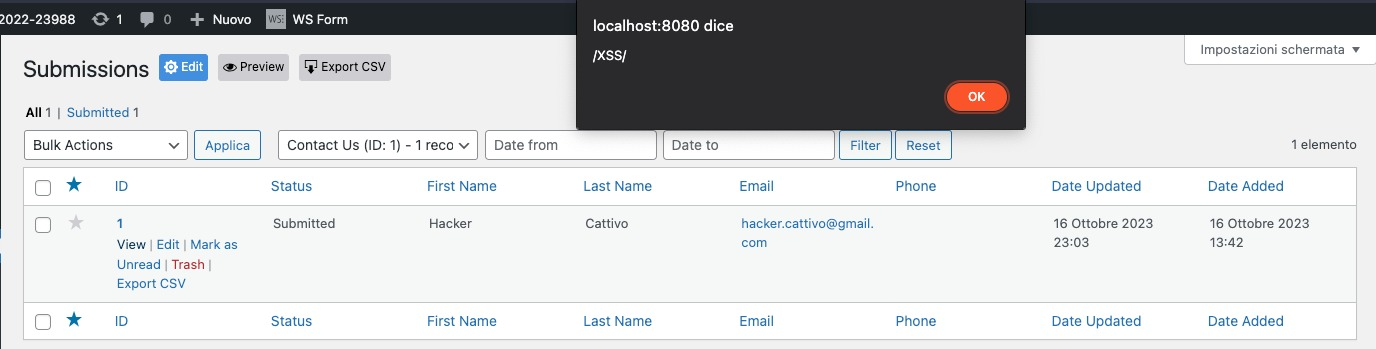
\includegraphics[width=1\textwidth]{XSS} 
	\end{figure}
	
	 
	\subsubsection{Mitigation}
	CVE-2022-23988 is fixed by escaping all user input before it is displayed on the website. This means that any characters that could be interpreted as HTML code are converted to their corresponding character entities. \\
	
	This escaping is done using functions provided by the programming languages or framework that is being used to develop the website. In wordpress, a plugin is a PHP file with a WordPress plugin header comment. Looking at the source code on \href{https://github.com/WordPress/WordPress/commit/948a260e805f11709cd38bf305a3092070ec7f66}{git hub} we can see that developers changed the PHP escaping function, from \verb|e()| to \verb|esc_attr_e()|. The main difference between \verb|e()| and \verb|esc_attr_e()| is that \verb|esc_attr_e()| escapes all HTML special characters in the string that is passed to it, meanwhile \verb|e()| does not escape any HTML special character.
	
	In addition, the community also developed a tool to help users identify and fix websites that are vulnerable to CVE-2022-23988, this is a plugin that scans websites and checks if the current version of plugins running is safe from known problems. 

\end{document}